\documentclass{article}
\usepackage{amsmath}
\usepackage[margin=1in]{geometry}
\usepackage{amsfonts}
\usepackage{hyperref}
\usepackage{graphicx}
\usepackage{amssymb}

\begin{document}
	
	\title{Eigenvectors}
	\author{Andy Chong Sam}
	
	\maketitle
	
	\section{Introduction}
	
	\par \noindent An \textbf{eigenvector} is a vector that preserves its direction in a transformation. A more formal definition is as follows - it is a nonzero vector \(\vec v\) such that \(A\vec v = \lambda \vec v\). In this formula, A is the transformation matrix, \( \vec v\) represents the vector input to the transformation and \(\lambda\) is a scalar called an \textbf{eigenvalue}. The intuition behind the more formal definition is that if indeed a vector's direction remains unchanged, then it should only differ from the transformation output in scaling.
	\newline
	\par \noindent The process to find an eigenvalue relies on a rearrangement of the definition we discussed:
	\begin{flalign*}
		A\vec v = \lambda \vec v \\
	\end{flalign*}
	\par \noindent Since \(\lambda \vec v\) is the same as \(\lambda \vec v I\), where \(I\) is a suitable identity matrix:
	\begin{flalign*}
				A\vec v - \lambda \vec v I = 0 \therefore \vec v (A - \lambda I) = 0
	\end{flalign*}
	\par\noindent Of particular interest is \(det( A - \lambda I) = 0\) as it produces a \textbf{characteristic polynomial}. The \( \lambda \) value that solves for this equation is the eigenvalue.
	\newline

	
	\section{Calculation}

	\par\noindent Eigenvector and Eigenvalue problems typically involve the following steps:
	\newline
	
	\begin{enumerate}
		\item Determine the vector \(A - \lambda I\)
		\item Derive the characteristic polynomial by taking the determinant of \(A - \lambda I\)
		\item Calculate the root(s) of the characteristic polynomial
		\item Substitute the root into \(\lambda\) for the vector obtained in step 1
		\item Simplify step 4 by using an augmented matrix
		\item Collect the eigenvector
	\end{enumerate}
	
	\newpage
	\section{Sheer Example}
		
	\par\noindent We saw in the linear transformation section an example of sheering:
	\[
	\left(\begin{array}{@{}cc@{}}
		1 & \frac{3}{2} \\
		0 & 1\\
	\end{array}\right)
	\]
	\par\noindent Evaluate \(A - \lambda I\):
	 \[
	 \left(\begin{array}{@{}cc@{}}
	 	1 & \frac{3}{2} \\
	 	0 & 1\\
	 \end{array}\right) - 
 	 \left(\begin{array}{@{}cc@{}}
 	\lambda & 0 \\
 	0 & \lambda\\
 \end{array}\right) = 
 	 \left(\begin{array}{@{}cc@{}}
	1 - \lambda & \frac{3}{2} \\
	0 & 1 - \lambda\\
\end{array}\right) 
	 \]
	 \par\noindent Evaluate \(det(A - \lambda I)\):
	 \[
	 	det(A - \lambda I) = (1 - \lambda)^2
	 \]
	 \par\noindent Determine the eigenvalue(s) \(\lambda\):
	 \begin{flalign*}
	 	(1 - \lambda)^2 = 0 \therefore \lambda = 1
	 \end{flalign*}
 \par \noindent Insert the eigenvalue(s) into \(A - \lambda I\):
 \[ 
\left(\begin{array}{@{}cc@{}}
1 - 1 & \frac{3}{2} \\
0 & 1 - 1\\
\end{array}\right) 
\left(\begin{array}{@{}c@{}}
	x \\
	y \\
\end{array}\right) 
=  
 \left(\begin{array}{@{}cc@{}}
 	0 & \frac{3}{2} \\
 	0 & 0\\
 \end{array}\right) 
 \left(\begin{array}{@{}c@{}}
 	x \\
 	y \\
 \end{array}\right) 
 \]
 \par\noindent Solve for \( \vec v\) in the system \( \vec v (A - \lambda I)\) = \( \vec 0\):
 \[
  \left(\begin{array}{@{}cc@{}}
 	0 & \frac{3}{2} \\
 	0 & 0\\
 \end{array}\right) \xrightarrow[]{\frac{2}{3}R_1 = R_1} 
  \left(\begin{array}{@{}cc@{}}
 	0 & 1 \\
 	0 & 0\\
 \end{array}\right) \xrightarrow[]{R_1 <-> R_2}
  \left(\begin{array}{@{}cc@{}}
	0 & 0 \\
	0 & 1\\
\end{array}\right)
\]
\par \noindent If \( \vec v = <x,y> \), then \(y=0\) and \(x \in \mathbb{R}\). In other words, any vector that has \(y=0\) and any value of x is a candidate to be an eigenvector. We typically report the simplest vector that meets this criteria, so \(<1,0>\) is an eigenvector.
\newline
\newline
\newline
\begin{minipage}[c]{.5\linewidth}
\par \noindent We can verify this answer by plugging in a vector that conforms to the description above (any real number for x, and 0 for y):
\[ 
\left(\begin{array}{@{}cc@{}}
	1 & \frac{3}{2} \\
	0 & 1\\
\end{array}\right) 
\left(\begin{array}{@{}c@{}}
	5 \\
	0 \\
\end{array}\right) 
=   
\left(\begin{array}{@{}c@{}}
	5 \\
	0 \\
\end{array}\right) 
\]
\par \noindent The resulting vector \(<5,0>\) differs from the eigenvector only by a factor, and thus it has the same direction as \(<1,0>\).
\newline
\par \noindent The transformation above is an example of a sheer. In the context of an image transformation, we can imagine that every vector shifts to the right or left only. On the image transformation below, the blue arrow will have the same direction as the transformed vector, differing only by scale.
\end{minipage}
\begin{minipage}[c]{.5\linewidth}
\begin{center}
	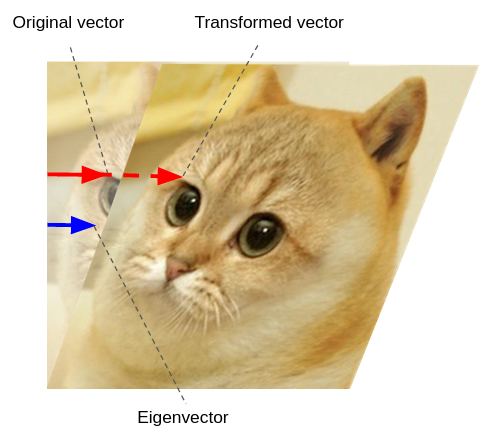
\includegraphics[width=6.5cm]{eigen-cate-sheered.png}	
\end{center}
\begin{center}
	\textbf{Figure 1}
\end{center}

\end{minipage}
\newline
\newline

\par \noindent Suppose \( \vec v = <-1,0>\). The transformation produces \(<-1,0>\). The eigenvector is still valid, as we can get \(<-1,0>\) by multiplying the eigenvector by -1. Although \( <-1,0> \) points in the opposite direction, in the mathematical sense, this is still considered scaling and not a change in direction. 
\newpage
\section {Vertical Scaling Example}
\par \noindent Previously we examined this transformation:

\[
\left(\begin{array}{@{}cc@{}}
	1 & 0 \\
	0 & \frac{3}{2} \\
\end{array}\right)
\]

\par\noindent Let's determine its eigenvalue and eigenvectors:
	\par\noindent Evaluate \(A - \lambda I\):
\[
\left(\begin{array}{@{}cc@{}}
	1 & 0 \\
	0 & \frac{3}{2}\\
\end{array}\right) - 
\left(\begin{array}{@{}cc@{}}
	\lambda & 0 \\
	0 & \lambda\\
\end{array}\right) = 
\left(\begin{array}{@{}cc@{}}
	1 - \lambda & 0 \\
	0 & \frac{3}{2} - \lambda\\
\end{array}\right) 
\]
\par\noindent Evaluate \(det(A - \lambda I)\):
\[
det(A - \lambda I) = (1 - \lambda)(\frac{3}{2} - \lambda)
\]
\par\noindent Determine the eigenvalue(s) \(\lambda\):
\begin{flalign*}
	\lambda = 1, \frac{3}{2}
\end{flalign*}
\par \noindent Determine the eigenvector for \(\lambda=1 \):
\[ 
\left(\begin{array}{@{}cc@{}}
	0 & 0 \\
	0 & \frac{3}{2} - 1 \\
\end{array}\right) 
\left(\begin{array}{@{}c@{}}
	x \\
	y \\
\end{array}\right) 
=  
\left(\begin{array}{@{}cc@{}}
	0 & 0 \\
	0 & \frac{1}{2}\\
\end{array}\right) 
\left(\begin{array}{@{}c@{}}
	x \\
	y \\
\end{array}\right) 
\]
\[
\left(\begin{array}{@{}cc@{}}
	0 & 0 \\
	0 & \frac{1}{2}\\
\end{array}\right) \xrightarrow[]{2R_2 = R_2} 
\left(\begin{array}{@{}cc@{}}
	0 & 0 \\
	0 & 1\\
\end{array}\right) \xrightarrow[]{R_1 <-> R_2}
\left(\begin{array}{@{}cc@{}}
	0 & 1 \\
	0 & 0\\
\end{array}\right)
\]
\par\noindent Given \(\vec v = <x,y>\), x can be any real number, but \(y\) has to equal 0. The eigenvector is \(<1,0>\). 
\newline
\par\noindent Determine the eigenvector for \(\lambda = \frac{3}{2}\):
\[ 
\left(\begin{array}{@{}cc@{}}
	1 - \frac{3}{2} & 0 \\
	0 & 0 \\
\end{array}\right) 
\left(\begin{array}{@{}c@{}}
	x \\
	y \\
\end{array}\right) 
=  
\left(\begin{array}{@{}cc@{}}
	-\frac{1}{2} & 0 \\
	0 & 0\\
\end{array}\right) 
\left(\begin{array}{@{}c@{}}
	x \\
	y \\
\end{array}\right) 
\]
\[
\left(\begin{array}{@{}cc@{}}
	-\frac{1}{2} & 0 \\
	0 & 0\\
\end{array}\right) \xrightarrow[]{-2R_2 = R_2} 
\left(\begin{array}{@{}cc@{}}
	1 & 0 \\
	0 & 0\\
\end{array}\right)
\]
\par\noindent Given \(\vec v = <x,y>\), x is zero, but \(y\) can be any real number. The eigenvector is \(<0,1>\).
\newline
\newline
\newline
\begin{minipage}[c]{.5\linewidth}
	\par \noindent We can spot check with an input vector that meets the above criteria, in this case \(<0,2>\) 
	\[ 
	\left(\begin{array}{@{}cc@{}}
		1 &  0 \\
		0 & \frac{3}{2}\\
	\end{array}\right) 
	\left(\begin{array}{@{}c@{}}
		0 \\
		2 \\
	\end{array}\right) 
	=   
	\left(\begin{array}{@{}c@{}}
		3 \\
		0 \\
	\end{array}\right) 
	\]
	\par \noindent The resulting vector \(<3,0>\) differs from the eigenvector \(<1,0>\) by only scaling. If we had plugged in \(<2,0>\) we would have obtained \(<2,0>\) which differs from the eigenvector \(<0,1>\) only by  scale.
\end{minipage}
\begin{minipage}[c]{.5\linewidth}
	\begin{center}
		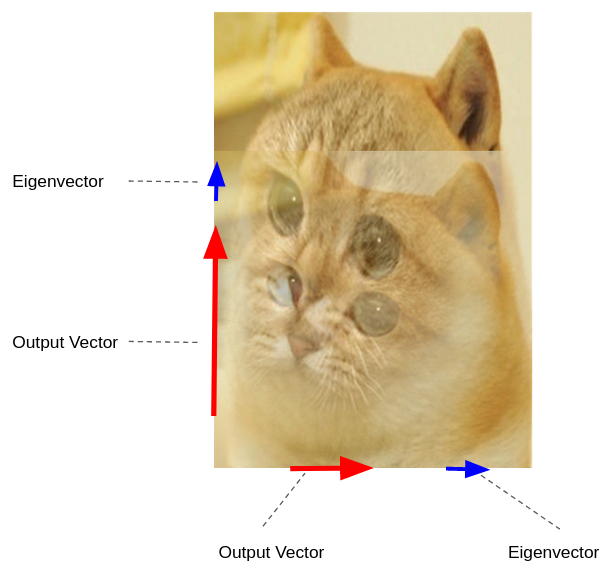
\includegraphics[width=6.5cm]{eigen-cate-scaled.png}	
	\end{center}
	\begin{center}
		\textbf{Figure 2}
	\end{center}

\end{minipage}
\newpage
\section {Additional Problems}
\framebox{
	\parbox{\linewidth}{
		\par \noindent \textbf{Ex. 1} Determine the eigenvalues and eigenvectors for matrix A:
		
		\[A=
			\left(\begin{array}{@{}cc@{}}
			0 &  1 \\
			-2 & -3 \\
		\end{array}\right) 
		\]
		\par \noindent First we determine the eigenvalues:
		\[
			A- \lambda I = 
			\left(\begin{array}{@{}cc@{}}
				- \lambda &  1 \\
				-2 & -3 - \lambda \\
			\end{array}\right) \therefore
		    det(A - \lambda I) = \lambda ^2 + 3 \lambda + 2 =
		    (\lambda + 2)( \lambda + 1)
		\]
		\par \noindent \textbf{We have two eigenvalues: -2 and -1}. 
		\newline
		\par \noindent We can start deriving the eigenvector starting with \(\lambda = -1\):
		\[
			A - (-1)I =
			\left(\begin{array}{@{}cc@{}}
				1  &  1 \\
				 -2 & -2 \\
			\end{array}\right) 
		\]
		\[
		\left(\begin{array}{@{}cc@{}}
			1  &  1 \\
			-2 & -2 \\
		\end{array}\right) \xrightarrow[]{-\frac{1}{2}R_2 = R_2}
	\left(\begin{array}{@{}cc@{}}
		1  &  1 \\
		1 & 1 \\
	\end{array}\right) \xrightarrow[]{R_1 - R_2 = R_1}
\left(\begin{array}{@{}cc@{}}
	1  &  1 \\
	0 & 0 \\
\end{array}\right)
		\]
		\par\noindent Given \( \vec v = (x,y)\) then the solution to the system is \(x + y = 0\) or \(x = -y\), where \(x,y \in \mathbb{R}\). Any vector that meets this criteria will work, so we pick the simplest. \textbf{The eigenvector is \(<1,-1>\).}
		\newline
		\par \noindent We now derive the eigenvector for \( \lambda = -2\):
		
		\[
		A-(-2)\lambda = 
			\left(\begin{array}{@{}cc@{}}
			2  &  1 \\
			-2 & -1 \\
		\end{array}\right) 
		\]
		\[
		A-(-2)\lambda = 
		\left(\begin{array}{@{}cc@{}}
			2  &  1 \\
			-2 & -1 \\
		\end{array}\right) \xrightarrow[]{R_2 + R_1 = R_2}
		\left(\begin{array}{@{}cc@{}}
			2  &  1 \\
			0 & 0 \\
		\end{array}\right)
		\]
		\par\noindent Given \( \vec v = (x,y)\), the solution to they system is \(2x + y =0\), or \(y = -2x\), where \(x,y \in \mathbb{R}\). \textbf{The eigenvector is \(<1,-2>\)}.
	}}

\end {document}